\documentclass[10pt,twocolumn,a4paper]{article}

\usepackage[utf8]{inputenc}
\usepackage[margin=1.8cm]{geometry}
\usepackage{amsmath,amssymb}
\usepackage{graphicx}
\usepackage{booktabs}
\usepackage{cite}
\usepackage{hyperref}
\usepackage{microtype}
\usepackage{xcolor}

\hypersetup{
    colorlinks=true,
    linkcolor=blue!70!black,
    citecolor=green!50!black,
    urlcolor=blue!80!black
}

\title{\textbf{Learned Page Replacement under Dynamic Workload Distribution Shift:\\An Empirical Operating Systems Evaluation}}
\author{
    \textbf{Student Name: Md Shamim Ahmed Limon \quad Student ID: 202414043}\\
    CSE-307: Operating Systems (Section B) Term Paper\\
    Department of Computer Science and Engineering
}
\date{October 2026}

\begin{document}

\maketitle

\begin{abstract}
Virtual memory management relies fundamentally on page replacement algorithms to minimize costly storage access latencies during page faults. While classical heuristic policies such as First-In, First-Out (FIFO) and Least Recently Used (LRU) rely on static assumptions regarding temporal and sequential locality, machine learning approaches aim to predict eviction candidates dynamically. In this study, we implement and benchmark four page replacement algorithms from scratch: FIFO, LRU, Belady's theoretical Optimal policy (MIN), and a lightweight Decision Tree-based Learned policy. Using a controlled synthetic benchmark of 2,000 page references with a deliberate midpoint distribution shift (transitioning from a locality-heavy working set to an erratic, bursty access pattern), we analyze algorithm resilience. Our experimental results show that in the locality-heavy phase, the Learned policy achieves a 59.60\% hit ratio, outperforming LRU (53.20\%) and FIFO (48.10\%). However, when subjected to the random/bursty second phase, the static Learned policy's hit ratio drops to 13.30\%, underperforming both LRU (21.60\%) and FIFO (21.50\%). These findings highlight the critical trade-off between predictive specialization and robustness to workload phase changes in learned operating system subsystems.
\end{abstract}

\section{Introduction}
Modern operating systems rely on paged virtual memory architectures to present applications with the abstraction of a vast, contiguous address space while operating within limited physical RAM~\cite{silberschatz2018operating}. When an active thread references a virtual page not currently resident in physical frames, the memory management unit triggers a hardware page fault exception, requiring the operating system to retrieve the missing page from backing store. Because secondary storage I/O is orders of magnitude slower than main memory access, page replacement algorithms strive to maximize the hit ratio and minimize fault frequencies~\cite{denning1968working}.

Traditional replacement policies employ fixed heuristics. FIFO evicts the oldest resident page regardless of usage history, whereas LRU exploits temporal locality by discarding the page unaccessed for the longest duration~\cite{silberschatz2018operating}. Although Belady's Optimal algorithm~\cite{belady1966study} provides the theoretical upper bound on replacement efficiency by evicting the page needed furthest in the future, it requires omniscient future knowledge and is impossible to implement directly in real-time kernels.

Recently, learned operating systems components have garnered substantial attention~\cite{vietri2018lecar}. By training machine learning models on offline execution traces, learned page replacement seeks to approximate Belady's decisions using historical state features. However, real-world application workloads undergo dramatic phase transitions, altering memory access distributions dynamically. 

This paper investigates whether a lightweight, explainable Decision Tree policy can effectively learn page eviction patterns, how it compares against classical baselines, and how it responds when the underlying access distribution undergoes a sudden shift.

\section{Background}
\subsection{Classical Replacement Policies}
\textbf{FIFO (First-In, First-Out):} Allocates a circular or queue structure to record page arrival. Upon a fault in a full frame set, the page loaded earliest is evicted. FIFO ignores access frequency and recency, making it vulnerable to evicting heavily accessed pages (and susceptible to Belady's Anomaly)~\cite{silberschatz2018operating}.

\textbf{LRU (Least Recently Used):} Exploits the principle of temporal locality by maintaining an ordering of access timestamps. When replacement is triggered, LRU evicts the page unreferenced for the longest time:
\begin{equation}
\text{victim}_{\text{LRU}} = \arg\min_{p \in \mathcal{F}} \big( \text{last\_access}(p) \big)
\end{equation}
where $\mathcal{F}$ represents the set of resident physical frames.

\textbf{Optimal (Belady's MIN):} Serves as an unachievable offline gold standard~\cite{belady1966study}. Belady proved that the minimum page fault rate is achieved by evicting the page whose next reference occurs furthest in the future:
\begin{equation}
\text{victim}_{\text{OPT}} = \arg\max_{p \in \mathcal{F}} \big( \text{next\_access}(p) \big)
\end{equation}

\subsection{Learned Eviction Concept}
A learned replacement policy models page eviction as a supervised classification problem~\cite{vietri2018lecar,pedregosa2011scikit}. Whenever physical frames are exhausted and an eviction is mandatory, the model evaluates each resident page $p \in \mathcal{F}$ based strictly on past access statistics, predicting the probability that $p$ aligns with the optimal victim.

\section{Methodology}
\subsection{Experimental Architecture}
To guarantee experimental integrity and avoid data leakage, our research methodology strictly isolates model training from evaluation, as illustrated in the pipeline architecture:
\begin{enumerate}
    \item \textbf{Training Workloads:} 5 independent synthetic traces (seeds 100--104) are generated.
    \item \textbf{Offline Oracle Generation:} Belady's algorithm simulates each training trace. At every eviction event, candidate feature vectors are extracted from past history and labeled ($y=1$ for the optimal victim, $y=0$ otherwise).
    \item \textbf{Model Induction:} A \texttt{DecisionTreeClassifier} (maximum depth = 4, balanced class weights) is fitted to the offline dataset.
    \item \textbf{Held-Out Evaluation:} A distinct evaluation workload (seed 42, length 2,000) containing an explicit midpoint shift is evaluated identically across FIFO, LRU, Optimal, and Learned policies.
\end{enumerate}

\subsection{Feature Formulation (Strict Past-Only)}
During inference, the model must make real-time decisions without any lookahead into future steps. For each resident page $p \in \mathcal{F}$ at step $t$, we compute a 4-dimensional feature vector:
\begin{enumerate}
    \item \textbf{Recency ($\Delta t$):} Steps elapsed since $p$ was last accessed: $t - \text{last\_access}(p)$.
    \item \textbf{Total Frequency ($f_{\text{tot}}$):} Cumulative references to $p$ since trace initialization.
    \item \textbf{Sliding-Window Frequency ($f_{\text{win}}$):} References to $p$ within the recent window $W = 50$ steps.
    \item \textbf{Resident Age ($a_{\text{res}}$):} Steps elapsed since $p$ entered physical memory: $t - \text{load\_time}(p)$.
\end{enumerate}

\subsection{Inference and Deterministic Tie-Breaking}
When a page fault occurs and $|\mathcal{F}| = K$ (allocated frames):
\begin{equation}
\text{victim} = \arg\max_{p \in \mathcal{F}} \Big( P(y=1 \mid \mathbf{x}_p) \Big)
\end{equation}
If multiple resident candidates share identical predicted probabilities, ties are broken deterministically by highest recency $\Delta t$, followed by lowest page identifier.

\begin{figure}[t]
    \centering
    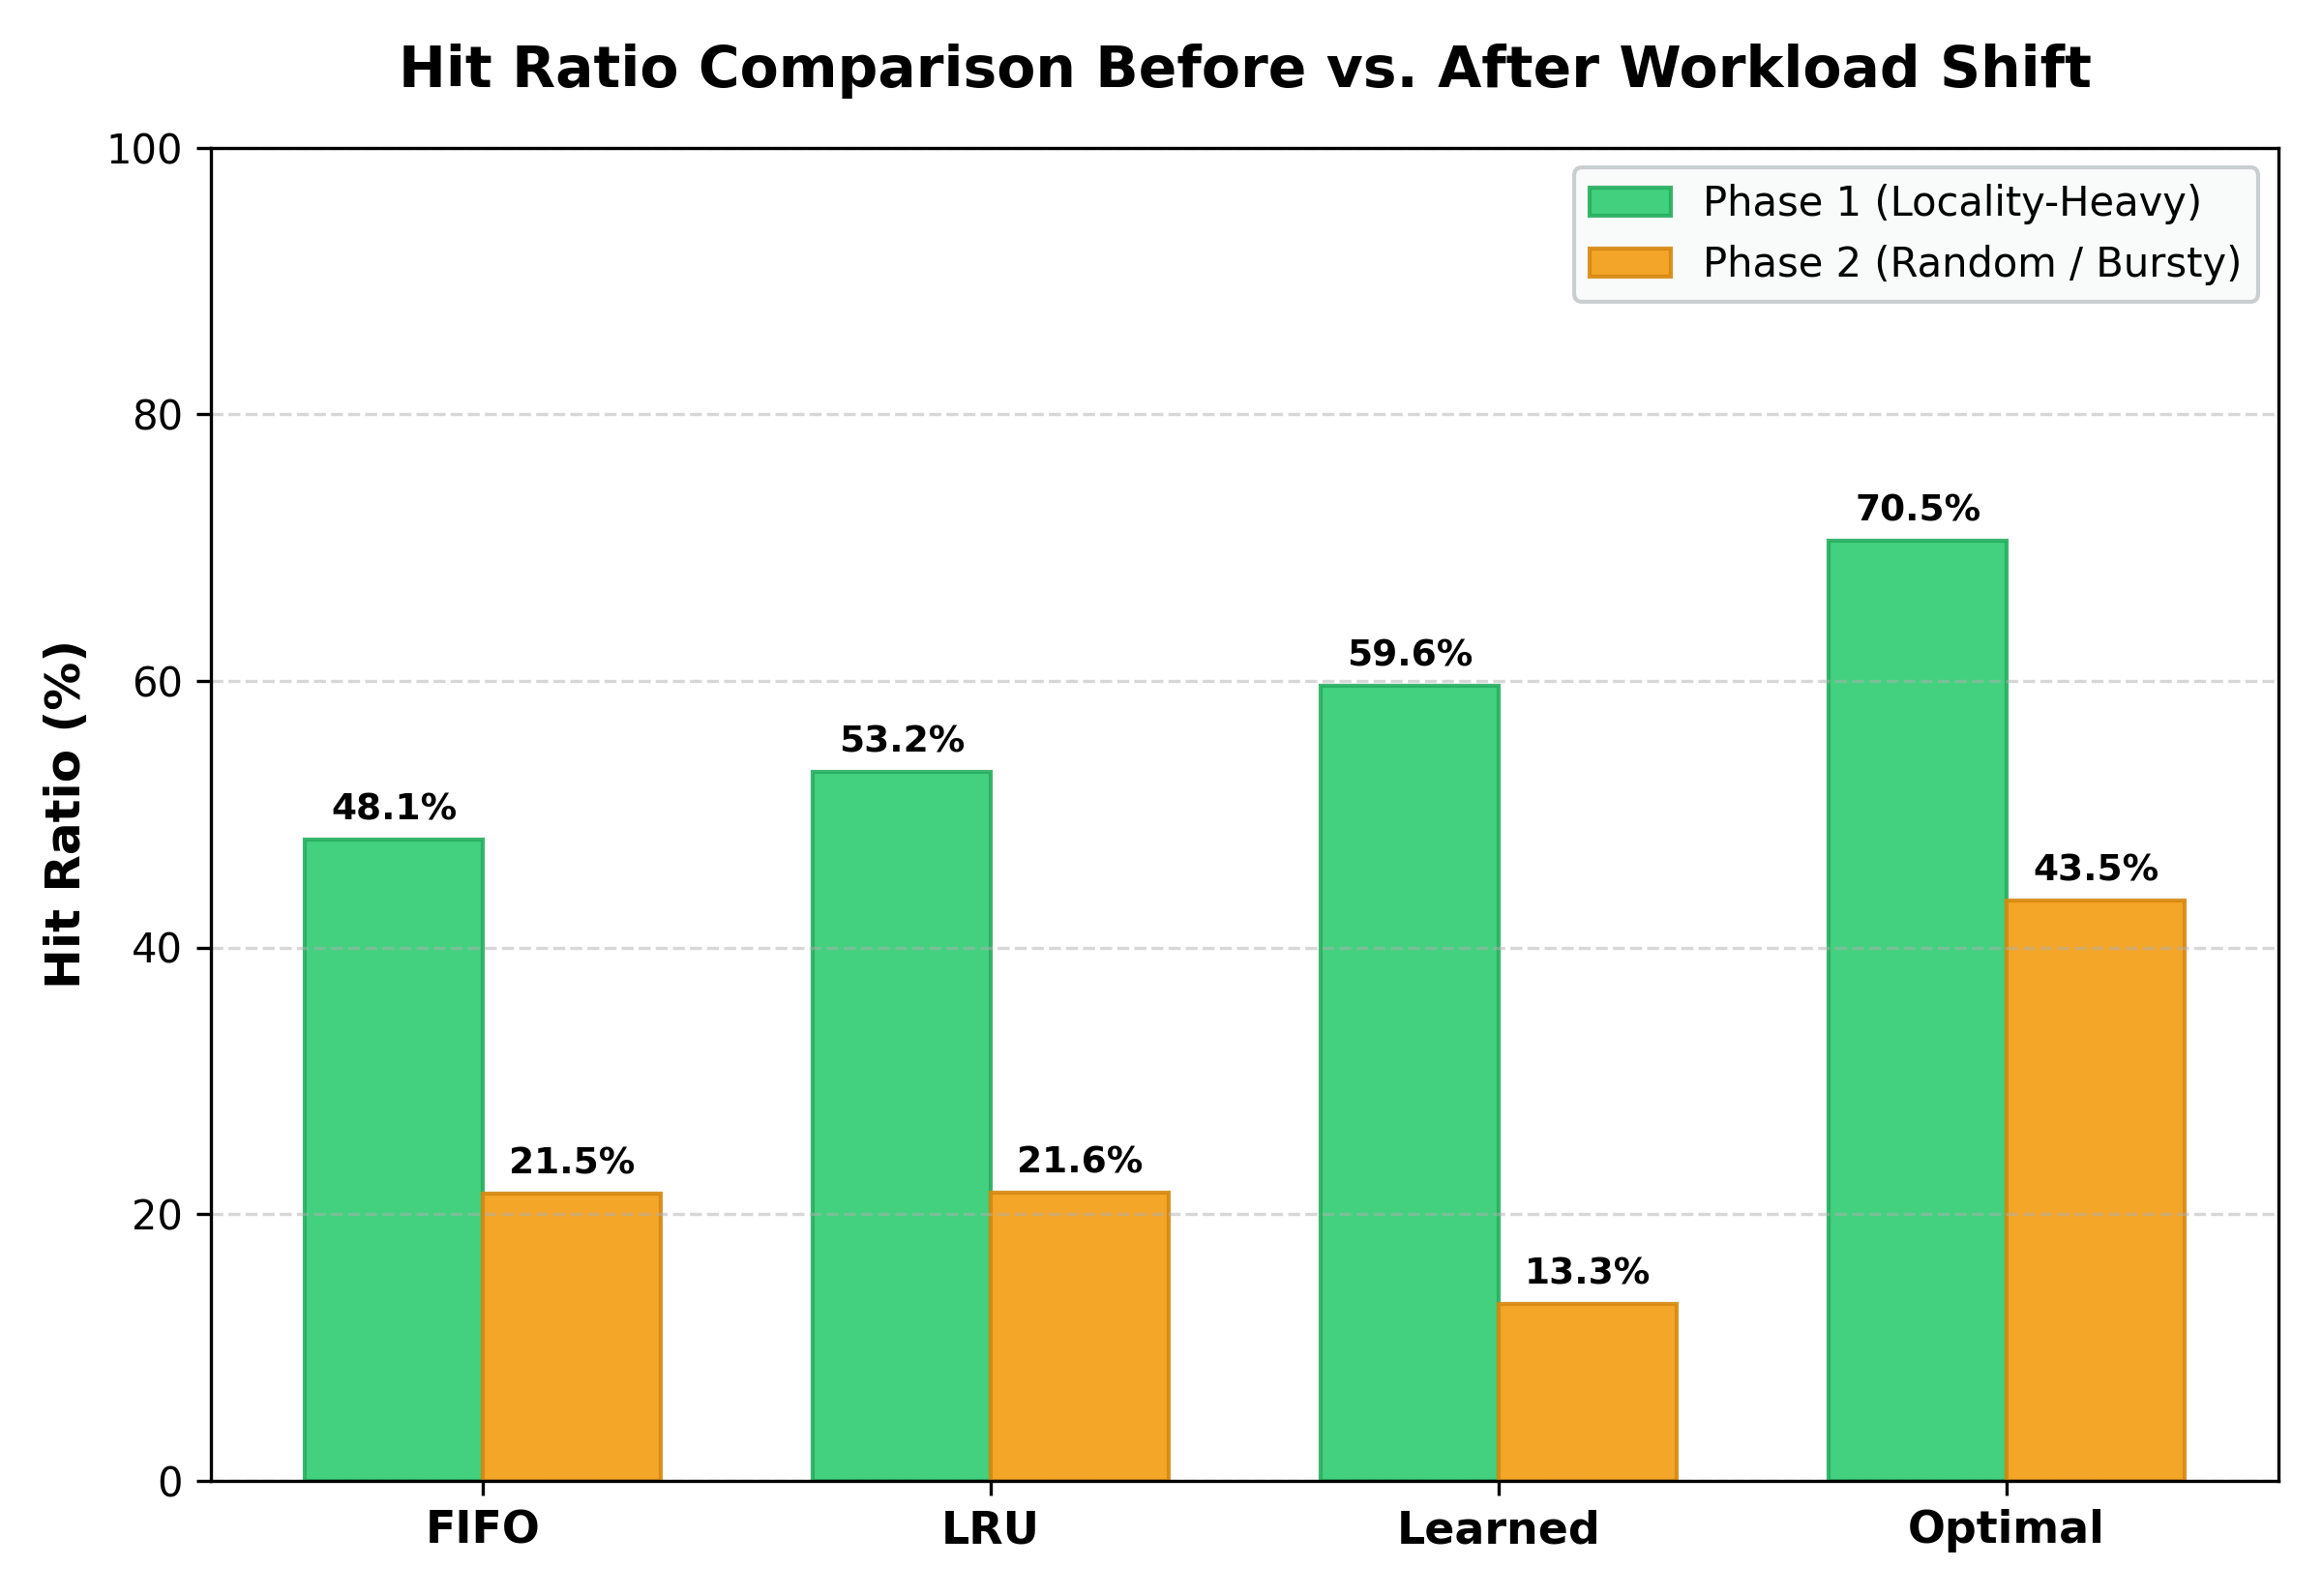
\includegraphics[width=\columnwidth]{../figures/hit_ratio_before_after.png}
    \caption{Hit ratio comparison across replacement algorithms before and after the midpoint workload shift ($K=5$ frames).}
    \label{fig:hit_ratio}
\end{figure}

\begin{figure}[t]
    \centering
    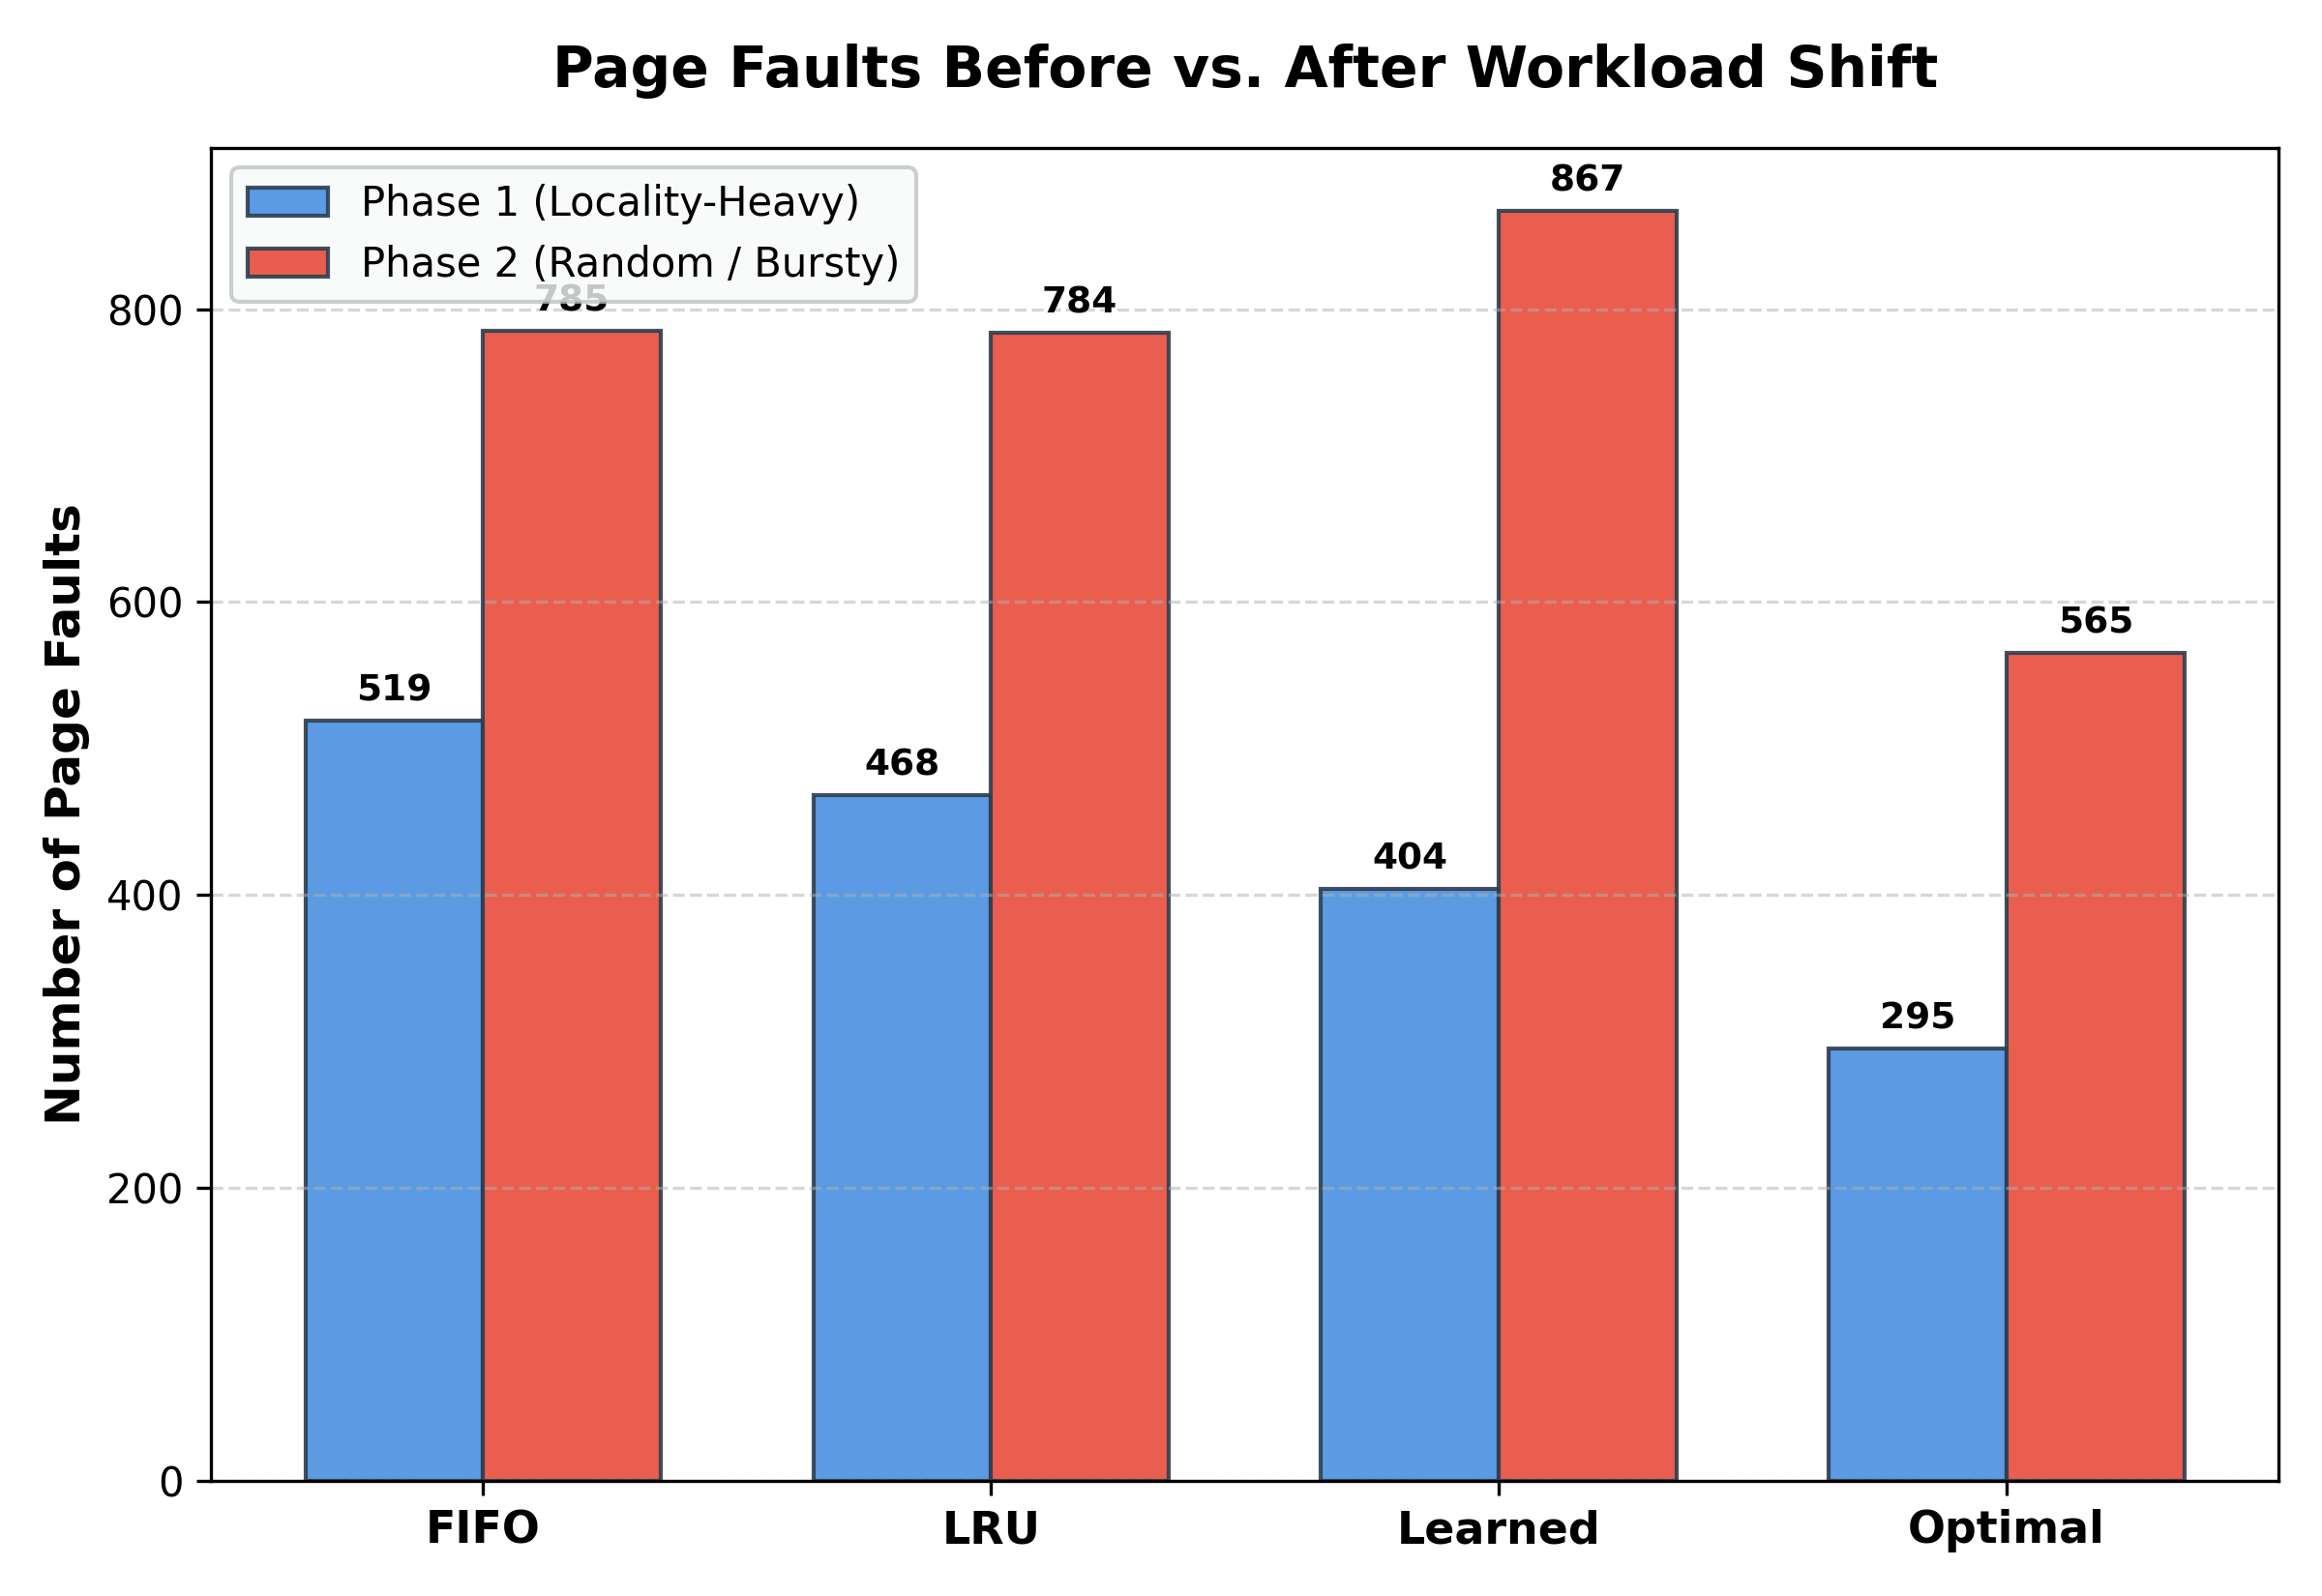
\includegraphics[width=\columnwidth]{../figures/page_faults_before_after.png}
    \caption{Total page fault counts before and after the workload shift.}
    \label{fig:page_faults}
\end{figure}

\subsection{Workload Shift Design}
The evaluation workload comprises $N = 2000$ references with a total universe of $M = 50$ virtual pages, partitioned at shift index $S = 1000$:
\begin{itemize}
    \item \textbf{Phase 1 (Steps 0--999, Locality-Heavy):} Accesses focus primarily on an active working set of 8 pages ($p \in [0, 7]$) with geometric repetition (65\% probability), sequential loops (20\%), and low noise (15\%).
    \item \textbf{Phase 2 (Steps 1000--1999, Random / Bursty):} The working set dissolves into dynamic 6-page bursts that switch unpredictably across the full 50-page universe (45\% probability), mixed with uniform random references across all 50 pages (55\%).
\end{itemize}

\section{Experimental Results}
Table~\ref{tab:summary_results} displays the measured empirical performance across all algorithms for a standard memory allocation of $K = 5$ frames. All results satisfy the exact mathematical identity: $\text{hits} + \text{page\_faults} = \text{references}$.

\begin{table}[h]
\centering
\small
\caption{Performance Metrics Segmented by Workload Phase}
\label{tab:summary_results}
\resizebox{\columnwidth}{!}{%
\begin{tabular}{llcccc}
\toprule
\textbf{Algorithm} & \textbf{Phase} & \textbf{Refs} & \textbf{Hits} & \textbf{Faults} & \textbf{Hit Ratio} \\
\midrule
FIFO    & Before Shift & 1000 & 481 & 519 & 48.10\% \\
        & After Shift  & 1000 & 215 & 785 & 21.50\% \\
        & Overall      & 2000 & 696 & 1304 & 34.80\% \\
\midrule
LRU     & Before Shift & 1000 & 532 & 468 & 53.20\% \\
        & After Shift  & 1000 & 216 & 784 & 21.60\% \\
        & Overall      & 2000 & 748 & 1252 & 37.40\% \\
\midrule
Learned & Before Shift & 1000 & 596 & 404 & \textbf{59.60\%} \\
(Tree)  & After Shift  & 1000 & 133 & 867 & 13.30\% \\
        & Overall      & 2000 & 729 & 1271 & 36.45\% \\
\midrule
Optimal & Before Shift & 1000 & 705 & 295 & \textbf{70.50\%} \\
(MIN)   & After Shift  & 1000 & 435 & 565 & 43.50\% \\
        & Overall      & 2000 & 1140 & 860 & \textbf{57.00\%} \\
\bottomrule
\end{tabular}%
}
\end{table}

\section{Discussion and Analysis}
\subsection{Phase 1: Learned Policy Performance}
In the first half of the trace, memory accesses exhibit clear spatial and temporal structure. LRU achieves a 53.20\% hit ratio by evicting pages with high recency values $\Delta t$. However, the Learned Decision Tree policy achieves a higher \textbf{59.60\%} hit ratio on this trace, reducing page faults from 468 to 404. 

The improvement is consistent with using several past-only signals rather than recency alone. However, aggregate hit/fault counts do not establish that a particular feature caused the gain, so the result should be interpreted as an empirical outcome of the complete learned policy rather than proof of a single causal mechanism.

\subsection{Phase 2: Distribution Shift and Model Drift}
Following step 1000, the access pattern shifts abruptly to unpredictable bursts across 50 pages. In this phase:
\begin{itemize}
    \item Optimal hit ratio declines from 70.50\% to 43.50\%, consistent with the second phase having weaker locality and a much larger active page universe.
    \item LRU and FIFO also decline to 21.60\% and 21.50\% respectively.
    \item The static Learned policy drops further to \textbf{13.30\%} hit ratio (867 faults).
\end{itemize}
The aggregate metrics alone do not prove that one feature caused this degradation. One plausible contributor is state-distribution mismatch: training labels are generated from resident-page states produced by the Optimal oracle, whereas during evaluation the learned policy's own earlier eviction decisions create different later candidate sets. The fixed tree is also not updated at the phase boundary. Because the training traces were generated from the same two-phase workload family, the second phase is best described as a workload phase shift rather than a completely unseen out-of-distribution workload.

\subsection{Frame Capacity Sensitivity}
We conducted an additional sensitivity analysis across frame counts $K \in \{3, 5, 7, 10\}$. At $K=3$, the Learned policy reaches a 27.85\% overall hit ratio versus LRU's 25.75\%. At $K=10$, however, LRU reaches 56.75\% while the Learned policy falls to 33.60\%. This shows that the learned policy is sensitive to frame capacity and that a model trained separately for each $K$ does not necessarily scale monotonically with additional frames.

\section{System and VM Resource Profiling Status}
The repository includes \texttt{scripts/run\_resource\_profile.sh} and an environment logger for collecting elapsed time, CPU time, and maximum resident set size under Ubuntu/VMware. These scripts keep the algorithmic workload and random seed fixed while the student manually changes the VM resource configuration. At the time of this report draft, those VM runs have not been executed; therefore, no system-level performance conclusions are claimed here.

\section{Conclusion}
This study found that the learned policy outperformed FIFO and LRU during the structured first phase, but it did not outperform LRU overall and degraded sharply after the workload phase shift. Optimal remained the strongest offline reference because it uses future knowledge. The results motivate future work on online adaptation, periodic retraining, or hybrid fallbacks that combine learned decisions with robust classical policies.

{\footnotesize
\bibliographystyle{plain}
\bibliography{references}
}

\end{document}
